%----------------------------------------------------------------------------------------
%	
%----------------------------------------------------------------------------------------

%----------------------------------------------------------------------------------------
%	CONFIGURACION DOCUMENTO
%----------------------------------------------------------------------------------------

\documentclass{article}

%%%%%%%%%%%%%%%%%%%%%%%%%%%%%%%%%%%%%%%%%
% Lachaise Assignment
% Structure Specification File
% Version 1.0 (26/6/2018)
%
% This template originates from:
% http://www.LaTeXTemplates.com
%
% Authors:
% Marion Lachaise & François Févotte
% Vel (vel@LaTeXTemplates.com)
%
% License:
% CC BY-NC-SA 3.0 (http://creativecommons.org/licenses/by-nc-sa/3.0/)
% 
%%%%%%%%%%%%%%%%%%%%%%%%%%%%%%%%%%%%%%%%%

%----------------------------------------------------------------------------------------
%	IDIOMA
%----------------------------------------------------------------------------------------

\usepackage[spanish]{babel}

%----------------------------------------------------------------------------------------
%	PACKAGES AND OTHER DOCUMENT CONFIGURATIONS
%----------------------------------------------------------------------------------------

\usepackage[table,xcdraw]{xcolor}
\usepackage{booktabs}

\usepackage{multicol}

\usepackage{multirow}

\usepackage{amsmath,amsfonts,stmaryrd,amssymb} % Math packages

\usepackage{enumerate} % Custom item numbers for enumerations

\usepackage[ruled]{algorithm2e} % Algorithms

\usepackage[framemethod=tikz]{mdframed} % Allows defining custom boxed/framed environments

\usepackage{listings} % File listings, with syntax highlighting
\lstset{
	basicstyle=\ttfamily, % Typeset listings in monospace font
}

%----------------------------------------------------------------------------------------
%	DOCUMENT MARGINS
%----------------------------------------------------------------------------------------

\usepackage{geometry} % Required for adjusting page dimensions and margins

\geometry{
	paper=a4paper, % Paper size, change to letterpaper for US letter size
	top=2cm, % Top margin
	bottom=2cm, % Bottom margin
	left=2cm, % Left margin
	right=2cm, % Right margin
	headheight=14.2pt, % Header height
	footskip=1.3cm, % Space from the bottom margin to the baseline of the footer
	headsep=0.8cm, % Space from the top margin to the baseline of the header
	%showframe, % Uncomment to show how the type block is set on the page
}

%----------------------------------------------------------------------------------------
%	FONTS
%----------------------------------------------------------------------------------------

\usepackage[utf8]{inputenc} % Required for inputting international characters
\usepackage[T1]{fontenc} % Output font encoding for international characters

\usepackage{XCharter} % Use the XCharter fonts

%----------------------------------------------------------------------------------------
%	COMMAND LINE ENVIRONMENT
%----------------------------------------------------------------------------------------

% Usage:
% \begin{commandline}
%	\begin{verbatim}
%		$ ls
%		
%		Applications	Desktop	...
%	\end{verbatim}
% \end{commandline}

\mdfdefinestyle{commandline}{
	leftmargin=10pt,
	rightmargin=10pt,
	innerleftmargin=15pt,
	middlelinecolor=black!50!white,
	middlelinewidth=2pt,
	frametitlerule=false,
	backgroundcolor=black!5!white,
	frametitle={Command Line},
	frametitlefont={\normalfont\sffamily\color{white}\hspace{-1em}},
	frametitlebackgroundcolor=black!50!white,
	nobreak,
}

\mdfdefinestyle{commandline2}{
	leftmargin=5pt,
	rightmargin=5pt,
	innerleftmargin=15pt,
	middlelinecolor=black!50!white,
	middlelinewidth=2pt,
	frametitlerule=false,
	backgroundcolor=black!5!white,
	frametitle={Command Line},
	frametitlefont={\normalfont\sffamily\color{white}\hspace{-1em}},
	frametitlebackgroundcolor=black!50!white,
	nobreak,
}
% Define a custom environment for command-line snapshots
\newenvironment{commandline}{
	\medskip
	\begin{mdframed}[style=commandline]
}{
	\end{mdframed}
	\medskip
}

\newenvironment{commandline22}{
	\medskip
	\begin{mdframed}[style=commandline2]
}{
	\end{mdframed}
	\medskip
}

%----------------------------------------------------------------------------------------
%	FILE CONTENTS ENVIRONMENT
%----------------------------------------------------------------------------------------

% Usage:
% \begin{file}[optional filename, defaults to "File"]
%	File contents, for example, with a listings environment
% \end{file}

\mdfdefinestyle{file}{
	innertopmargin=1.6\baselineskip,
	innerbottommargin=0.8\baselineskip,
	topline=false, bottomline=false,
	leftline=false, rightline=false,
	leftmargin=2cm,
	rightmargin=2cm,
	singleextra={%
		\draw[fill=black!10!white](P)++(0,-1.2em)rectangle(P-|O);
		\node[anchor=north west]
		at(P-|O){\ttfamily\mdfilename};
		%
		\def\l{3em}
		\draw(O-|P)++(-\l,0)--++(\l,\l)--(P)--(P-|O)--(O)--cycle;
		\draw(O-|P)++(-\l,0)--++(0,\l)--++(\l,0);
	},
	nobreak,
}

% Define a custom environment for file contents
\newenvironment{file}[1][File]{ % Set the default filename to "File"
	\medskip
	\newcommand{\mdfilename}{#1}
	\begin{mdframed}[style=file]
}{
	\end{mdframed}
	\medskip
}

%----------------------------------------------------------------------------------------
%	NUMBERED QUESTIONS ENVIRONMENT
%----------------------------------------------------------------------------------------

% Usage:
% \begin{question}[optional title]
%	Question contents
% \end{question}

\mdfdefinestyle{question}{
	innertopmargin=1.2\baselineskip,
	innerbottommargin=0.8\baselineskip,
	roundcorner=5pt,
	nobreak,
	singleextra={%
		\draw(P-|O)node[xshift=1em,anchor=west,fill=white,draw,rounded corners=5pt]{%
		Question \theQuestion\questionTitle};
	},
}

\newcounter{Question} % Stores the current question number that gets iterated with each new question

% Define a custom environment for numbered questions
\newenvironment{question}[1][\unskip]{
	\bigskip
	\stepcounter{Question}
	\newcommand{\questionTitle}{~#1}
	\begin{mdframed}[style=question]
}{
	\end{mdframed}
	\medskip
}

%----------------------------------------------------------------------------------------
%	WARNING TEXT ENVIRONMENT
%----------------------------------------------------------------------------------------

% Usage:
% \begin{warn}[optional title, defaults to "Warning:"]
%	Contents
% \end{warn}

\mdfdefinestyle{warning}{
	topline=false, bottomline=false,
	leftline=false, rightline=false,
	nobreak,
	singleextra={%
		\draw(P-|O)++(-0.5em,0)node(tmp1){};
		\draw(P-|O)++(0.5em,0)node(tmp2){};
		\fill[black,rotate around={45:(P-|O)}](tmp1)rectangle(tmp2);
		\node at(P-|O){\color{white}\scriptsize\bf !};
		\draw[very thick](P-|O)++(0,-1em)--(O);%--(O-|P);
	}
}

% Define a custom environment for warning text
\newenvironment{warn}[1][Warning:]{ % Set the default warning to "Warning:"
	\medskip
	\begin{mdframed}[style=warning]
		\noindent{\textbf{#1}}
}{
	\end{mdframed}
}

%----------------------------------------------------------------------------------------
%	INFORMATION ENVIRONMENT
%----------------------------------------------------------------------------------------

% Usage:
% \begin{info}[optional title, defaults to "Info:"]
% 	contents
% 	\end{info}

\mdfdefinestyle{info}{%
	topline=false, bottomline=false,
	leftline=false, rightline=false,
	nobreak,
	singleextra={%
		\fill[black](P-|O)circle[radius=0.4em];
		\node at(P-|O){\color{white}\scriptsize\bf i};
		\draw[very thick](P-|O)++(0,-0.8em)--(O);%--(O-|P);
	}
}

% Define a custom environment for information
\newenvironment{info}[1][Info:]{ % Set the default title to "Info:"
	\medskip
	\begin{mdframed}[style=info]
		\noindent{\textbf{#1}}
}{
	\end{mdframed}
}


\usepackage[table]{xcolor}
\usepackage{colortbl}

%----------------------------------------------------------------------------------------
%	INFORMACION
%----------------------------------------------------------------------------------------

\title{\textbf{Laboratorio 1: }Administrador de Procesos --- Parte A\@: Procesos y Comunicación Entre Procesos}


\author{ \textbf{Integrantes: }
Facundo Nicolás Farias Lozano,
Juan Cruz Paez,
Tomás Agustín Muñoz.
}

\date{\textbf{Docentes: } 
Mg. Cs. Molina Silvia, Dra. Natalia Miranda, Mg. Palacio Gabriela.\\
  \vspace{0.3cm}
  Sistemas Operativos\\ 
  \vspace{0.2cm}
  Universidad Nacional de San Luis\\
  \vspace{0.2cm}
  2025
  }

%\date{Universidad Nacional de San Luis --- 2025}

%----------------------------------------------------------------------------------------

\begin{document}

\maketitle

%----------------------------------------------------------------------------------------
%	RESOLUCIÓN
%----------------------------------------------------------------------------------------

\section*{Ejercicio 1: Acerca de Linux}

\begin{figure}[h]
  \centering
  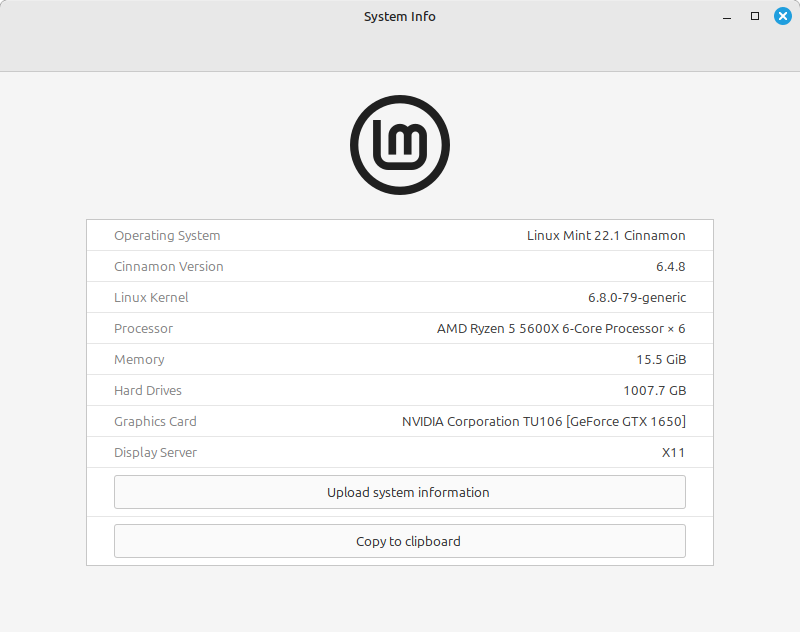
\includegraphics[width=0.85\textwidth]{resources/ej1a.png}
  \caption{System info}
\end{figure}

\subsection*{a- ¿Qué Sistema Operativo tiene instalado? ¿Qué distribución? ¿Qué versión?}
\noindent
El sistema operativo que se encuentra instalado es \textit{Linux Mint 22.1 Cinnamon} y es la version \textit{6.4.8}

\subsection*{b- ¿Cuántos procesadores posee su sistema de computadora? ¿Cuáles son sus características?}
\noindent
El sistema cuenta con un procesador \textit{AMD Ryzen 5 5600X}, el cual posee \textit{6 núcleos físicos y 12 hilos 
lógicos}, arquitectura \textit{Zen 3} y frecuencia base de \textit{3.7 GHz} hasta \textit{4.6 Ghz}

\subsection*{c- ¿Cuál es la capacidad de memoria disponible?}
\noindent
La memoria disponible es de \textit{15.5 GiB}.

\subsection*{d- ¿Qué placa de video o gráfica posee?}
\noindent
La placa de vídeo es la \textit{GeForce GTX 1650 NVIDIA}.\@

\subsection*{e- ¿Cuál es la capacidad de disco que posee?}
\noindent
La capacidad de disco con la que se cuenta es de \textit{1007.7 GB}.\@

%----------------------------------------------------------------------------------------

\section*{Ejercicio 2: Monitor de sistema}

\begin{figure}[h]
  \centering
  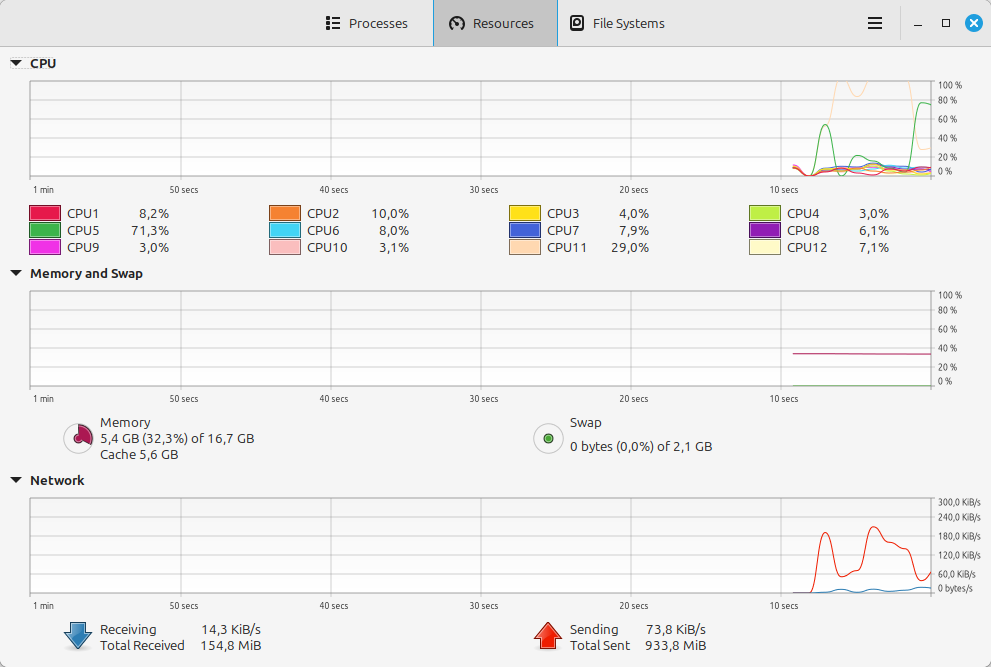
\includegraphics[width=0.85\textwidth]{resources/2.png}
  \caption{System monitor}
\end{figure}

\subsection*{a- ¿Qué información del sistema muestra?}

\noindent
Al abrir el \textit{monitor de sistema} podemos observar:

\begin{itemize}
    \item \textbf{Uso de la CPU:} Muestra un histograma del uso de los procesador en tiempo real.
    \item \textbf{Uso de la memoria y espacio intercambiado (swap)\footnote{Herramienta de gestión de memoria que actua cuando la memoria RAM física se llena}: }
    Muestra de forma gráfica el uso de la memoria RAM y el espacio de intercambio.
    \item \textbf{Actividad de Red: } Muestra de manera gráfica la transmisión de  datos de red.
\end{itemize}

\subsection*{b- Mencione y describa qué información relevante sobre “Procesos” se puede mostrar (pestaña de “Procesos”).}

\begin{figure}[h]
  \centering
  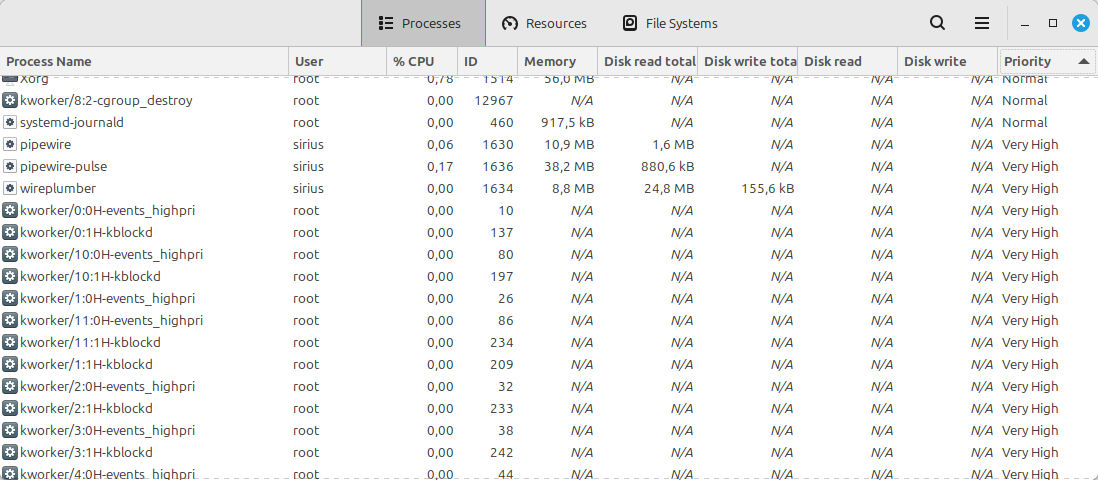
\includegraphics[width=0.85\textwidth]{resources/ej2b2.png}
  \caption{System monitor: Process}
\end{figure}

\begin{figure}[h]
  \centering
  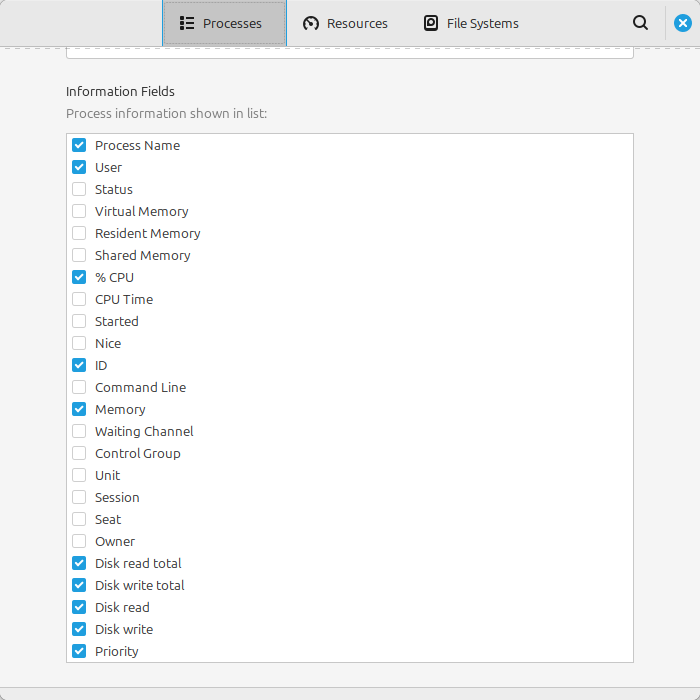
\includegraphics[width=0.5\textwidth]{resources/ej2b.png}
  \caption{System monitor: informacion de procesos}
\end{figure}

\noindent
En dicha pestaña se muestra informacion en tiempo real de todos los procesos activos en el sistema. De ellos podemos ver:
\begin{itemize}
  \item \textbf{Nombre de Proceso: }Indica el programa que esta ejecutando
  \item \textbf{Usuario:} Indica que usuario inicio el proceso.
  \item \textbf{Uso de CPU:} Porcentaje del procesador que esta consumiendo el proceso
  \item \textbf{Id:} Numero unico que identifica a cada proceso
  \item \textbf{Memoria:} Cantidad de memoria RAM que esta consumiendo el proceso
  \item \textbf{Lectura de disco:} Cantidad de informacion leida desde el disco por el proceso
  \item \textbf{Escritura de disco:} Cantidad de informacion escrita en el disco por el proceso
  \item \textbf{Prioridad:} Indica que priorida le da el sistema al proceso frente a otros.
  \item \textbf{Estado:} Indica si el proceso esta durmiendo, ejecutandose,etc
\end{itemize}

\noindent
Además, desde la pestaña procesos se agrega la posibilidad de mostrar información util como \textbf{CPU Time} y \textbf{Waiting Channel}.
\subsection*{c- ¿Qué operaciones se permite hacer respecto a los procesos?}

\noindent
Las operaciones que se permiten hacer sobre un proceso son:
\begin{itemize}
  \item \textbf{Open Files}
  \item \textbf{Change Priority}
  \item \textbf{Set Affinity}
  \item \textbf{Stop}
  \item \textbf{continue}
  \item \textbf{Terminate}
  \item \textbf{Memory Maps}
  \item \textbf{Kill}
  \item \textbf{End Procesos}
  \item \textbf{Show Process Properties}
\end{itemize}

\subsection*{d- ¿Cómo se muestran las prioridades de un proceso?}

\noindent
Las prioridades se muestran en una columna dedicada, donde cada proceso (fila) puede tomar los valores de: \textit{Very High}, \textit{High}, \textit{Normal}, 
\textit{Low}, \textit{Very Low}, \textit{Custom}

\subsection*{e- Inicializar las siguientes aplicaciones: un navegador Web, un procesador de texto y una
terminal/consola, luego responda observando la pestaña “Procesos” del Monitor de sistema:}


% Table generated by Excel2LaTeX from sheet 'Sheet1'
% chktex 44
\begin{table}[htbp]
  \centering
  % \caption{Información del monitor del sistema} No me convence como queda :(
    \begin{tabular}{|lrlll|}
    \toprule
    \rowcolor[rgb]{ .357,  .608,  .835} \textcolor[rgb]{ 1,  1,  1}{\textbf{Nombre Proceso}} & \multicolumn{1}{l}{\textcolor[rgb]{ 1,  1,  1}{\textbf{PID}}} & \textcolor[rgb]{ 1,  1,  1}{\textbf{Estado}} & \textcolor[rgb]{ 1,  1,  1}{\textbf{Ejecutando}} & \textcolor[rgb]{ 1,  1,  1}{\textbf{Tipo Cola}} \\
    \midrule
    \rowcolor[rgb]{ .867,  .922,  .969} bash  & 8039  & Sleeping & No    & do\_select \\
    \midrule
    brave & 10361 & Running & Si    & futex\_wait\_queue \\
    \midrule
    \rowcolor[rgb]{ .867,  .922,  .969} xed   & 15517 & Sleeping & No    & do\_poll.constprop.0 \\
    \bottomrule
    \end{tabular}%
  \label{tab:monitor_sistema}%
\end{table}%
 % chktex 44
 
 \begin{warn}[]
    \noindent
    Al detener un proceso, este permanece en memoria pero suspendido, sin posibilidad de ejecutarse hasta que se lo 
    reanude. Al finalizarlo, se envía una señal para que concluya de manera ordenada, aunque en algunos casos el
    proceso puede ignorar dicha señal. En cambio, al matarlo se fuerza su terminación inmediata, sin posibilidad de ser evitada.
 \end{warn}


\subsection*{f- Desde la pestaña “Procesos”, ordene los procesos por número de proceso, donde se muestren los
siguientes datos (identificador del procesos, nombre del proceso, usuario, propietario, estado,
prioridad, memoria real):}

\begin{figure}[h]
  \centering
  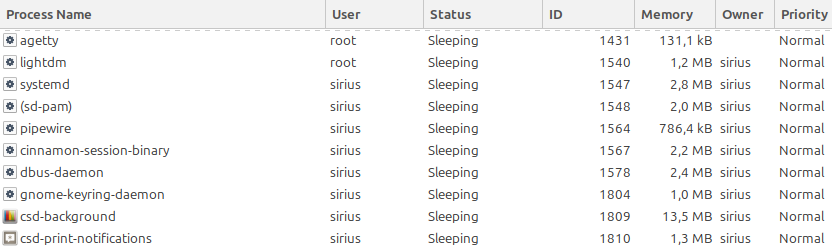
\includegraphics[width=1\textwidth]{resources/ej2f.png}
  \caption{System monitor: informacion de procesos}
\end{figure}

% Table generated by Excel2LaTeX from sheet 'Sheet1'
\begin{table}[htbp]
  \centering
    \begin{tabular}{|rrllllll|}
    \toprule
    \rowcolor[rgb]{ .357,  .608,  .835} \multicolumn{1}{|l}{\textcolor[rgb]{ 1,  1,  1}{\textbf{Proceso}}} & \multicolumn{1}{l}{\textcolor[rgb]{ 1,  1,  1}{\textbf{PID}}} & \textcolor[rgb]{ 1,  1,  1}{\textbf{Nombre Proceso}} & \textcolor[rgb]{ 1,  1,  1}{\textbf{Usuario}} & \textcolor[rgb]{ 1,  1,  1}{\textbf{Propietario}} & \textcolor[rgb]{ 1,  1,  1}{\textbf{Estado}} & \textcolor[rgb]{ 1,  1,  1}{\textbf{Prioridad}} & \textcolor[rgb]{ 1,  1,  1}{\textbf{Memoria}} \\
    \midrule
    \rowcolor[rgb]{ .867,  .922,  .969} 1     & 1431  & agetty & root  & $-$     & Sleeping & Normal & 131,1 kB \\
    \midrule
    3     & 1647  & systemd & root  & siruis & Sleeping & Normal & 2,8 MB \\
    \midrule
    \rowcolor[rgb]{ .867,  .922,  .969} 5     & 1564  & pipewire & sirius & siruis & Sleeping & Normal & 786,4 kB \\
    \midrule
    7     & 1678  & dbus-daemon & sirius & siruis & Sleeping & Normal & 2,4 MB \\
    \midrule
    \rowcolor[rgb]{ .867,  .922,  .969} 9     & 1809  & csd-background & sirius & siruis & Sleeping & Normal & 13,5 MB \\
    \bottomrule
    \end{tabular}%
  \label{tab:addlabel}%
\end{table}%

%----------------------------------------------------------------------------------------

\section*{Ejercicio 3: Simulador de Planificador de procesos}

\subsection*{a- ¿Qué partes del diagrama del ciclo de vida de un proceso se pueden visualizar en la ventana
principal?}

\noindent
En el diagrama de ejecución podemos observar los estados del ciclo de vida

\begin{itemize}
  \item \textbf{New}
  \item \textbf{Ready}
  \item \textbf{Running}
  \item \textbf{Bloqued}
  \item \textbf{Exit}
\end{itemize}

\subsection*{b- ¿Qué información de los procesos puede ser visualizada? Ejemplifique.}
\begin{figure}[h]
  \centering
  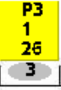
\includegraphics[width=0.1\textwidth]{resources/3b.png}
  \caption{Información de un proceso en el simulador}
\end{figure}

\noindent
Analizando la imagen, podemos obtener distintos datos sobre cada proceso, por ejemplo:

\begin{itemize}
  \item \textbf{P3:} indica el nombre o identificador del proceso.
  \item \textbf{1:} representa el número de ráfagas restantes que el proceso debe ejecutar.
  \item \textbf{26:} muestra la cantidad de unidades de tiempo que le faltan para completar la ráfaga actual.
  \item \textbf{3:} indica la prioridad asignada al proceso dentro del sistema.
\end{itemize}

\subsection*{c- Respecto a la configuración de la simulación. ¿Qué información de los procesos se puede configurar?}

\noindent
La información que se puede configurar para los procesos incluye:
\begin{itemize}
  \item \textbf{Algoritmo de planificación} a utilizar y, si corresponde, la especificación del quantum.
  \item \textbf{Llegadas de los procesos}, que pueden simularse según distintas distribuciones de probabilidad: 
  uniforme, exponencial, normal o Poisson.
  \item \textbf{Instante de llegada} de cada proceso.
  \item \textbf{Prioridad} asignada a cada proceso.
  \item \textbf{Número de ráfagas} que debe ejecutar el proceso.
  \item \textbf{Tipo y duración} de cada ráfaga (CPU o E/S).
  \item \textbf{Limitaciones de las ráfagas}, pudiendo restringirlas específicamente para E/S o CPU.\@
\end{itemize}

\subsection*{d- ¿Qué información importante se puede observar una vez ejecutada la simulación?}

\noindent
Al acceder a la pestaña Resultados, encontramos tres secciones distintas que proporcionan información valiosa:
\textit{Estadisticas}
permite consultar información detallada de la simulación. Incluye datos específicos de cada proceso, como instante de llegada,
prioridad, número de ráfagas, tiempo de espera, entre otros. Además, muestra estadísticas globales propias de toda la simulación.

\begin{figure}[h]
  \centering
  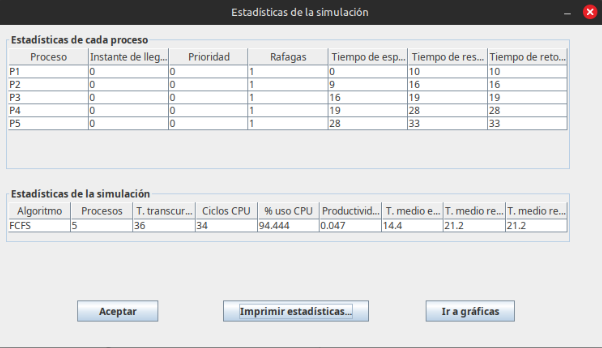
\includegraphics[width=0.7\textwidth]{resources/3dEst.png}
  \caption{Estadísticas específicas y globales}
\end{figure}

\noindent
\textbf{Comparación}
En esta sección se presentan los datos globales de cada simulación realizada, facilitando el análisis comparativo entre
diferentes ejecuciones.
\begin{figure}[h]
  \centering
  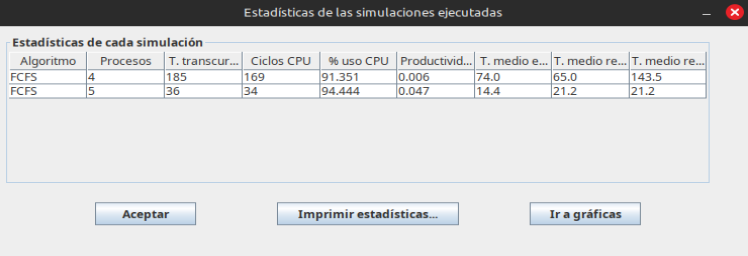
\includegraphics[width=0.7\textwidth]{resources/3dComp.png}
  \caption{Comparación de simulaciones}
\end{figure}

\noindent
\textbf{Gráficos}
Permite visualizar de manera gráfica los datos anteriormente mencionados, tanto los específicos de cada proceso como las
estadísticas globales de cada simulación.\footnote{\textbf{Nota:} Todas las imágenes presentadas corresponden a los resultados obtenidos a partir de la 
simulación utilizando los datos de la Tabla 1.}

\begin{figure}[h]
  \centering
  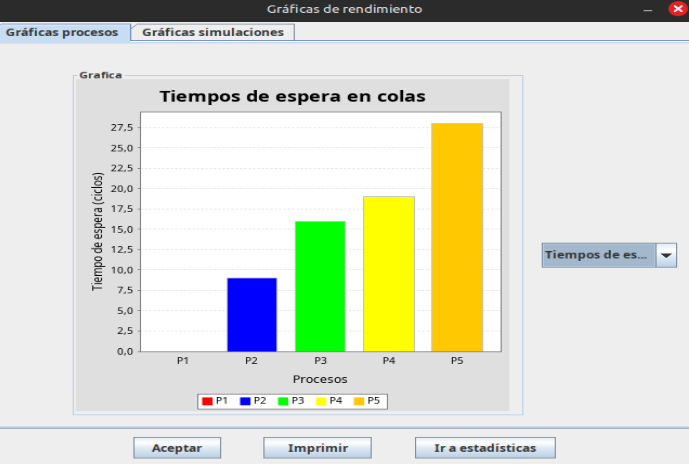
\includegraphics[width=0.49\textwidth]{resources/3dGra1.png}
  \hfill
  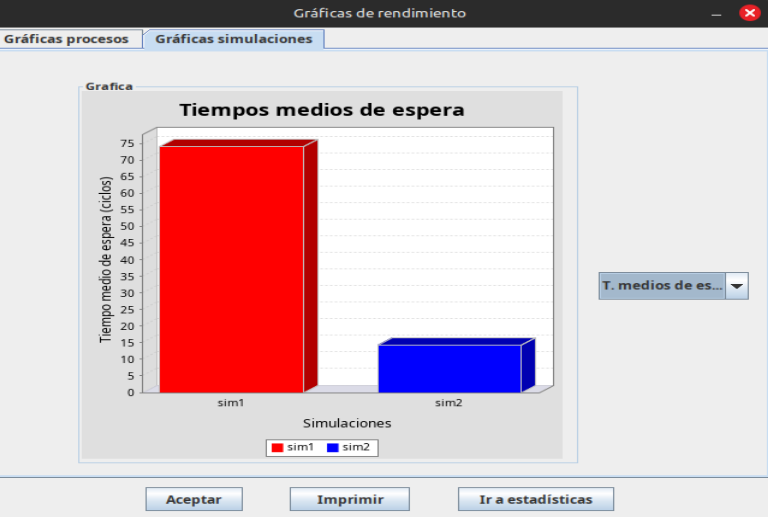
\includegraphics[width=0.49\textwidth]{resources/3dGra2.png}
  \caption{Izquierda: Gráfico de tiempo de espera en cola \quad | \quad Derecha: Tiempos medios de espera}
\end{figure}
\vfil


%----------------------------------------------------------------------------------------
\

\section*{Ejercicio 4: Inicialice la aplicación Terminal de Linux}


\subsection*{a- Utilizando el comando ps listar los procesos del sistema.}

\begin{commandline}
	\begin{verbatim}
	tomas@tomas-HP-245-G7-Notebook-PC:~$ ps
    PID TTY           TIME CMD
  10820 pts/0       00:00:00 bash
  10828 pts/0       00:00:00 ps
	\end{verbatim}
\end{commandline}

\subsection*{b- Utilizando el comando ps con el parámetro -u listar los procesos del usuario actual únicamente.}

\begin{commandline}
  \begin{verbatim}
  tomas@tomas-HP-245-G7-Notebook-PC:~$ ps -u
      USER      PID %CPU %MEM    VSZ   RSS TTY     STAT START      TIME COMMAND
      tomas    10820 0.0  0.0  14060  5248 pts/0   Ss   11:00      0:00 bash
      tomas    10861 100  0.0  16492  4608 pts/0   R+   11:02      0:00 ps -u
  \end{verbatim}
\end{commandline}


\subsection*{c- Utilizando el comando top listar los procesos.}

\begin{commandline}
 {\footnotesize
\begin{verbatim}
top - 11:05:42 up 2:04, 1 user,  load average: 1,82, 1,58, 1,72
Tareas: 249 total, 1 ejecutar, 248 hibernar, 0 detener, 0 zombie
%Cpu s: 15,2 us, 3,9 sy, 0,0 ni, 80,3 id, 0,1 wa, 0,0 hi, 0,5 si, 0,0 st
MiB Mem: 5835,5 total, 898,8 libre, 2940,5 usado, 2320,9 búf/caché
MiB Intercambio: 2048,0 total, 1618,2 libre, 429,8 usado. 2895,0 dispon Mem
PID  USUARIO   PR  NI     VIRT     RES     SHR S  %CPU  %MEM    HORA+   ORDEN
5365 tomas     20   0  1398,9g  538740  179392 S  52,5   9,0  84:04.65  Discord
5277 tomas     20   0    32,6g  166108  129620 S  13,3   2,8  14:16.99  Discord
2220 root      20   0  1303608  160792   95956 S   3,3   2,7  10:06.64  Xorg
2694 tomas      9 -11   162348   34900   11204 S   2,7   0,6   4:23.31  pipewire-pulse
3122 tomas     20   0  4942804  275096  120592 S   2,7   4,6  11:39.49  cinnamon
631  root     -51   0        0       0       0 S   2,3   0,0   2:58.75  irq/45-rtw88_pci
2690 tomas      9 -11   126460   16084    9264 S   1,7   0,3   3:19.48  pipewire
1    root      20   0    22988   13312    9216 S   0,7   0,2   0:02.93  systemd
1162 root      35  15     9816    6664    2304 S   0,3   0,1   0:03.52  preload
2251 mysql     20   0  2375904  254476   10496 S   0,3   4,3   0:56.81  mysqld
2788 tomas     20   0   312236    6144    5888 S   0,3   0,1   0:00.33  xdg-permission-
3817 tomas     20   0    32,9g  367464  253916 S   0,3   6,1   3:51.85  brave
3953 tomas     20   0  1394,0g  439296  145652 S   0,3   7,4   7:00.65  brave
5149 tomas     20   0  1392,1g  176052  136860 S   0,3   2,9   1:35.70  Discord
10288 root     20   0        0       0       0 I   0,3   0,0   0:11.34  kworker/u32:1-gfx_low
10659 root     20   0        0       0       0 I   0,3   0,0   0:00.09  kworker/u33:4-rtw_tx_wq
10895 tomas    20   0   545576   43008   34288 S   0,3   0,7   0:00.38  gnome-terminal-
10940 tomas    20   0    17348    6016    3840 R   0,3   0,1   0:00.07  top
2    root      20   0        0       0       0 S   0,0   0,0   0:00.01  kthreadd 
3    root      20   0        0       0       0 S   0,0   0,0   0:00.00  pool workqueue_release
4    root       0 -20        0       0       0 I   0,0   0,0   0:00.00  kworker/R-rcu_g
5    root       0 -20        0       0       0 I   0,0   0,0   0:00.00  kworker/R-rcu_p
6    root       0 -20        0       0       0 I   0,0   0,0   0:00.00  kworker/R-slub
7    root       0 -20        0       0       0 I   0,0   0,0   0:00.00  kworker/R-netns
10   root       0 -20        0       0       0 I   0,0   0,0   0:00.00  kworker/0:0H-events_highpri
12   root       0 -20        0       0       0 I   0,0   0,0   0:00.00  kworker/R-mm_pe
13   root      20   0        0       0       0 I   0,0   0,0   0:00.00  rcu_tasks_kthread
14   root      20   0        0       0       0 I   0,0   0,0   0:00.00  rcu_tasks_rude-kthread
15   root      20   0        0       0       0 I   0,0   0,0   0:00.00  rcu_tasks_trace-kthreadd
16   root      20   0        0       0       0 S   0,0   0,0   0:00.49  ksoftirqd/0
17   root      20   0        0       0       0 I   0,0   0,0   0:18.40  rcu_preempt
18   root      rt   0        0       0       0 S   0,0   0,0   0:00.03  migration/0
\end{verbatim}
}
\end{commandline}

\subsection*{d- ¿Cuál es la diferencia de utilizar el comando top respecto de utilizar el comando ps?}

\noindent
El comando \textit{ps} muestra el estado de los procesos de un momento determinado, es estático, es decir que no se actualiza automaticamente.

\noindent
Por otra parte, el comando \textit{top} muestra de manera interactiva y en tiempo real como cambia el estado de los procesos.

\subsection*{e- Observe la estructura jerárquica de los procesos en Linux utilizando el comando pstree.}

\begin{commandline}
 {
\begin{verbatim}
systemd-+-ModemManager---3*[{ModemManager}]
        |-NetworkManager---3*[{NetworkManager}]
        |-accounts-daemon---3*[{accounts-daemon}]
        |-agetty
        |-at-spi2-registr---3*[{at-spi2-registr}]
        |-avahi-daemon---avahi-daemon
        |-bluetoothd
        |-2*[chrome_crashpad---2*[chrome_crashpad]]
        |-chrome_crashpad---{chrome_crashpad}
        |-colord---3*[{colord}]
        |-cron
        |-csd-printer---3*[{csd-printer}]
        |-cups-browsed---3*[{cups-browsed}]
        |-cupsd
        |-dbus-daemon
        |-fwupd---5*[{fwupd}]
        |-irqbalance---{irqbalance}
        |-2*[kerneloops]
        `-lightdm-+-Xorg---12*[{Xorg}]
                 `-lightdm-+-cinnamon-session---agent---3*[{agent}]
                           |-at-spi-bus-laun---dbus-daemon---4*[{at-spi-bu+}]
                           |-caribou---3*[{caribou}]
                           |-cinnamon-killer---4*[{cinnamon-}]
                           |-cinnamon-launch---cinnamon---27+[{cinnamon}]
                           `-csd-ally-settin---6*[{cinnamon+}]
                                               `-4*[{csd-ally-+}]
\end{verbatim}
}
\end{commandline}

\noindent
Este comando muestra los procesos de manera que, indica cuales son \textit{padres} y cuales \textit{hijos}.
\textit{System} es el primer proceso que ejecuta linux y este va ser el padre de casi todos los demas.
Podemos observar que algunos de sus hijos son \textit{modem manager}, \textit{network manager}, \textit{accounts-daemon}, etc
\subsection*{f- Ejecute el comando htop, luego visualice los estados de los procesos a través de la columna S (state).}


\begin{commandline}
  {\scriptsize
    \begin{verbatim}
    Here's the transcription of the information displayed in the htop interface:
    Header Section:
    CPUs: Multiple CPU usage meters (graphical bars with percentages, e.g., |||||||20.0%, SHR S, etc.)
    Mem: [|||||||||||||||2.75G/5.700] (Memory usage: 2.75GB used out of 5.700GB total)
    Swp: [|||50M/2.00G] (Swap usage: 50MB used out of 2.00GB total)
    Tasks: 147, 759 thr, 122 kthr; 3 running
    Load average: 1.37 2.10 1.93
    Uptime: 02:27:03
    Process List (with column headers):
    PID   USER      PRI NI   VIRT   RES   SHR S CPU% MEM%   TIME+  Command
    13617 tomas      20 0   7228M 5564M  3072 R 4.5  8.1   0:09.63 /snap/htop/5092/usr/local/bin/htop
       1  root       20 0   22988  1696  9216 S 0.0  0.2   0:04.32 /sbin/init splash
     291  root       19 -1  83736 33436 32156 S 0.0  8.6   0:02.45 /usr/lib/systemd/systemd-journald
     362  root       20 0   30632  6204  4748 S 0.0  8.1   0:04.87 /usr/lib/systemd/systemd-udevd
     781  systemd-re 20 0   22480 12544 10624 S 0.0  0.2   0:00.37 /usr/lib/systemd/systemd-resolved
     799  systemd-ti 20 0   91212  7296   912 S 0.0  0.1   0:00.18 /usr/lib/systemd/systemd-timesyncd
     845  systemd-ti 20 0   91212  7296     0 S 0.0  0.1   0:00.00 /usr/lib/systemd/systemd-timesyncd
     999  root       20 0    309M  7388   124 S 0.0  0.1   0:00.00 /usr/libexec/accounts-daemon
    1000  root       20 0    309M  7388     0 S 0.0  0.1   0:00.00 /usr/libexec/accounts-daemon
    1001  root       20 0    309M  7388     0 S 0.0  0.1   0:00.52 /usr/libexec/accounts-daemon
    1003  avahi      20 0    6616  3968  3840 S 0.0  0.1   0:00.20 avahi-daemon: running[tomas-HP-245-G7-Notebook-PC.local]
    1005  root       20 0   13544  5632  5248 S 0.0  0.1   0:00.12 /usr/libexec/bluetooth/bluetoothd
    1006  root       20 0   12048   688   560 S 0.0  0.0   0:00.02 /usr/sbin/cron -f -P
    1007  messagebus 20 0  6100S6  6656   352 S 0.0  0.1   0:02.43 @dbus-daemon --system --address=systemd: --nofork 
    --nopidfile --systemd-activation --syslog-only
    1015  root       20 0   82920  3712   584 S 0.0  0.1   0:00.76 /usr/sbin/irqbalance
    1035  polkitd    20 0    155M 11988   524 S 0.0  0.2   0:00.57 /usr/lib/polkit-1/polkitd --no-debug
    1038  root       20 0   82920  3712     0 S 0.0  0.1   0:00.00 /usr/sbin/irqbalance
    1039  root       20 0    309M  7552     0 S 0.0  0.1   0:00.11 /usr/libexec/power-profiles-daemon
    1046  root       20 0   19508 30444 10512 S 6.9  0.5   0:02.19 /usr/lib/snapd/snapd
    1047  root       20 0    305M  6400   272 S 0.0  0.1   0:00.06 /usr/libexec/switcheroo-control
    1048  root       20 0    309M  7388     0 S 0.0  0.1   0:00.01 /usr/libexec/accounts-daemon
    1050  root       20 0   10148  6212   808 S 0.0  0.1   0:00.43 /usr/lib/systemd/systemd-logind
    1062  root       20 0    253M 14208 12416 S 0.0  0.2   0:16.34 /usr/bin/touchegg-daemon
    1064  root       20 0    308M  7552     0 S 0.0  0.1   0:00.00 /usr/libexec/power-profiles-daemon
    1065  root       20 0    308M  7552     0 S 0.0  0.1   0:00.00 /usr/libexec/power-profiles-daemon
    1067  root       20 0    308M  7552     0 S 0.0  0.1   0:00.00 /usr/libexec/power-profiles-daemon
    1083  root       20 0    458M 11568  9776 S 0.0  0.2   0:00.22 /usr/libexec/udisks2/udisksd
    1089  root       20 0    305M  6400     0 S 0.0  0.1   0:00.00 /usr/libexec/switcheroo-control
    1090  root       20 0    305M  6400     0 S 0.0  0.1   0:00.00 /usr/libexec/switcheroo-control
    Footer Menu:
    F1Help F2Setup F3Search F4Filter F5Tree F6Sortby F7Nice- F8Nice+ F9Kill F10Quit
    \end{verbatim}
  }
\end{commandline}

\noindent
La columna \textit{S} que resulta del comando \textit{htop} muestra el estado de un proceso.  

\subsection*{g- Utilizando el comando kill listar las opciones de parámetros posibles utilizando el parámetro -l, luego
investigue qué parámetros son necesarios para matar un proceso, muestre un ejemplo donde elige
un proceso para matar y luego lo mata aplicando el comando con los parámetros correspondiente.}

\noindent
Listamos todas las señales posibles con el comando \textit{kill-l}.

\begin{commandline}
 {
\begin{verbatim}
  tomas@tomas-HP-245-G7-Notebook-PC:~$ kill -l
  1) SIGHUP       2) SIGINT       3) SIGQUIT      4) SIGILL       5) SIGTRAP 
  6) SIGABRT      7) SIGBUS       8) SIGFPE       9) SIGKILL     10) SIGUSR1
 11) SIGSEGV     12) SIGUSR2     13) SIGPIPE     14) SIGALRM     15) SIGTERM
 16) SIGSTKFLT   17) SIGCHLD     18) SIGCONT     19) SIGSTOP     20) SIGTSTP
 21) SIGTTIN     22) SIGTTOU     23) SIGURG      24) SIGXCPU     25) SIGXFSZ
 26) SIGVTALRM   27) SIGPROF     28) SIGWINCH    29) SIGIO       30) SIGPWR   
 31) SIGSYS      34) SIGRTMIN    35) SIGRTMIN+1  36) SIGRTMIN+2  37) SIGRTMIN+3 
 38) SIGRTMIN+4  39) SIGRTMIN+5  40) SIGRTMIN+6  41) SIGRTMIN+7  42) SIGRTMIN+8 
 43) SIGRTMIN+9  44) SIGRTMIN+10 45) SIGRTMIN+11 46) SIGRTMIN+12 47) SIGRTMIN+13 
 48) SIGRTMIN+14 49) SIGRTMIN+15 50) SIGRTMAX-14 51) SIGRTMAX-13 52) SIGRTMAX-12 
 53) SIGRTMAX-11 54) SIGRTMAX-10 55) SIGRTMAX-9  56) SIGRTMAX-8  57) SIGRTMAX-7 
 58) SIGRTMAX-6  59) SIGRTMAX-5  60) SIGRTMAX-4  61) SIGRTMAX-3  62) SIGRTMAX-2 
 63) SIGRTMAX-1  64) SIGRTMAX
\end{verbatim}
}
\end{commandline}

\noindent
Cada número o nombre representa una señal que podés enviar a un proceso.

\medbreak\noindent
Las más usadas para terminar procesos son:

\begin{itemize}
  \item \textbf{SIGTERM} \textit{(15)} → Finalización ordenada: consiste en solicitar al proceso que termine su ejecución, 
  permitiéndole cerrar archivos, guardar datos, liberar memoria y limpiar recursos antes de finalizar. Sin embargo, el proceso 
  puede optar por ignorar la señal y no terminar con su ejecución.
  \item \textbf{SIGKILL} \textit{(9)} → Finalización forzada: se solicita al proceso que termine de manera inmediata y obligatoria,
  sin darle la posibilidad de cerrar archivos abiertos, liberar recursos o guardar datos. En este caso, el proceso no puede 
  ignorar la señal y debe finalizar.
\end{itemize}

\noindent
Veamos un ejemplo de uso:

\bigbreak\noindent
Listamos los procesos usando el comando \textit{top}
   
\begin{commandline}
 {
\begin{verbatim}
   PID  USUARIO PR  NI     VIRT    RES    SHR S %CPU %MEM     HORA+ ORDEN
  3122  tomas   20   0  4945876 240424 122640 S  6,6  4,0  14:00.76 cinnamon
 11227  tomas   20   0  3050700 332584 194800 S  4,6  5,6   1:12.07 spotify
  5365  tomas   20   0  1398,9g 394004 121524 S  3,0  6,6  93:20.76 Discord
  2694  tomas    9 -11   162324  35600  11264 S  2,0  0,6   5:14.95 pipewire-pulse
\end{verbatim}
}
\end{commandline}

\noindent
Mataremos el proceso Discord el cual tiene como PID 5365:

\medskip\noindent
Para finalizar amigablemente, se debe usar \textit{-SIGTERM} ó -15 equivalentemente.
    
\begin{commandline}
  \begin{verbatim}
    tomas@tomas-HP-245-G7-Notebook-PC:-$ kill -15 5365
  \end{verbatim}
\end{commandline}

\noindent
En caso de que el programa no finalice procedemos a usar -9 o \textit{-SIGKILL}.


\begin{commandline}
  \begin{verbatim}
    tomas@tomas-HP-245-G7-Notebook-PC:-$ kill -9 5365
    bash: killK (5365) - No existe el proceso
  \end{verbatim}
\end{commandline}

\noindent
En este caso, el mensaje se refiere a que el proceso no existe porque fue eliminado anteriormente con \textit{SIGTERM}.

%----------------------------------------------------------------------------------------

\end{document}